\section{Massa en lading uit knoopstructuur}

In het Vortex Æther Model ontstaan massa en lading als emergente grootheden uit de energie en heliciteit van de vortexknoop. De massa $M$ van een
vortexknoop kan berekend worden door de kinetische energie van de wervelstroming te integreren over het volume~\cite{Moffatt1990VortexHelicity}:
\begin{equation}
    E = \frac{1}{2}\int \rho_\text{\ae}\, v^2 \,dV, \qquad M = \frac{E}{c^2}.
\end{equation}

Hoewel een exacte integratie voor complexe knopen lastig is, leidt VAM tot een benaderende formule die massa recht evenredig met de heliciteit maakt. Zo wordt voor elementaire deeltjes (fermion-knopen) afgeleid:
\begin{equation}
    M \approx 8\pi \rho_\text{\ae} r_c^3 C_e \cdot L_k,
\end{equation}


% --- Figuur 5: Energie vs Heliciteit ---
\begin{figure}[H]
    \centering
    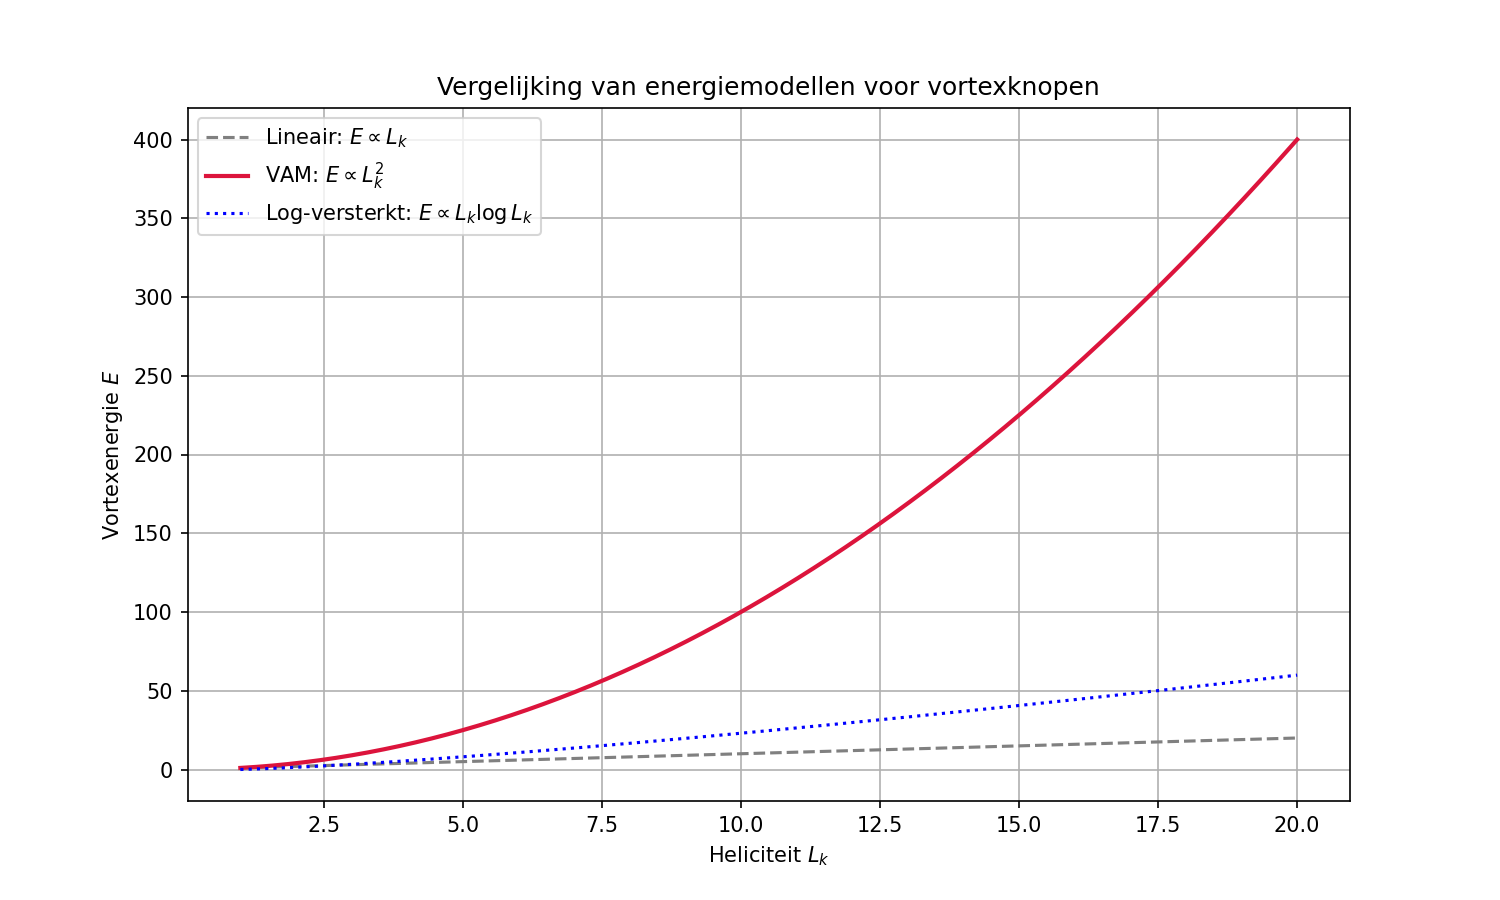
\includegraphics[width=0.7\textwidth]{../5_Wervelveldenergie}
    \caption{Vortexenergie $E$ als functie van heliciteit $L_k$ onder verschillende benaderingen. Het kwadratische VAM-model wijkt af van lineaire klassieke benaderingen.}
    \label{fig:energie_vs_heliciteit}
\end{figure}

waar $L_k$ de topologische linking number (heliciteit quanta) van de knoop is. Deze formule toont dat elke winding/linking extra inertiële massa bijdraagt. Voor de trefoilknoop ($L_k=3$) krijgen we $M \approx 8\pi \rho_\text{\ae} r_c^3 C_e \cdot 3$. Met de waarden uit Tabel 1 levert dit numeriek een massa in de juiste orde van grootte voor nucleonen (zij het dat hier fijnafstemming nodig is om exact de protonmassa te krijgen – zie Discussie). Het belangrijke punt is dat massa topologisch verankerd is: hoe ingewikkelder de knoop (hoe hoger $L_k$), des te groter de totale vortexenergie die opgeslagen zit in het wervelveld.

% --- Figuur 6: Chiraliteit en lading ---
\begin{figure}[H]
    \centering
    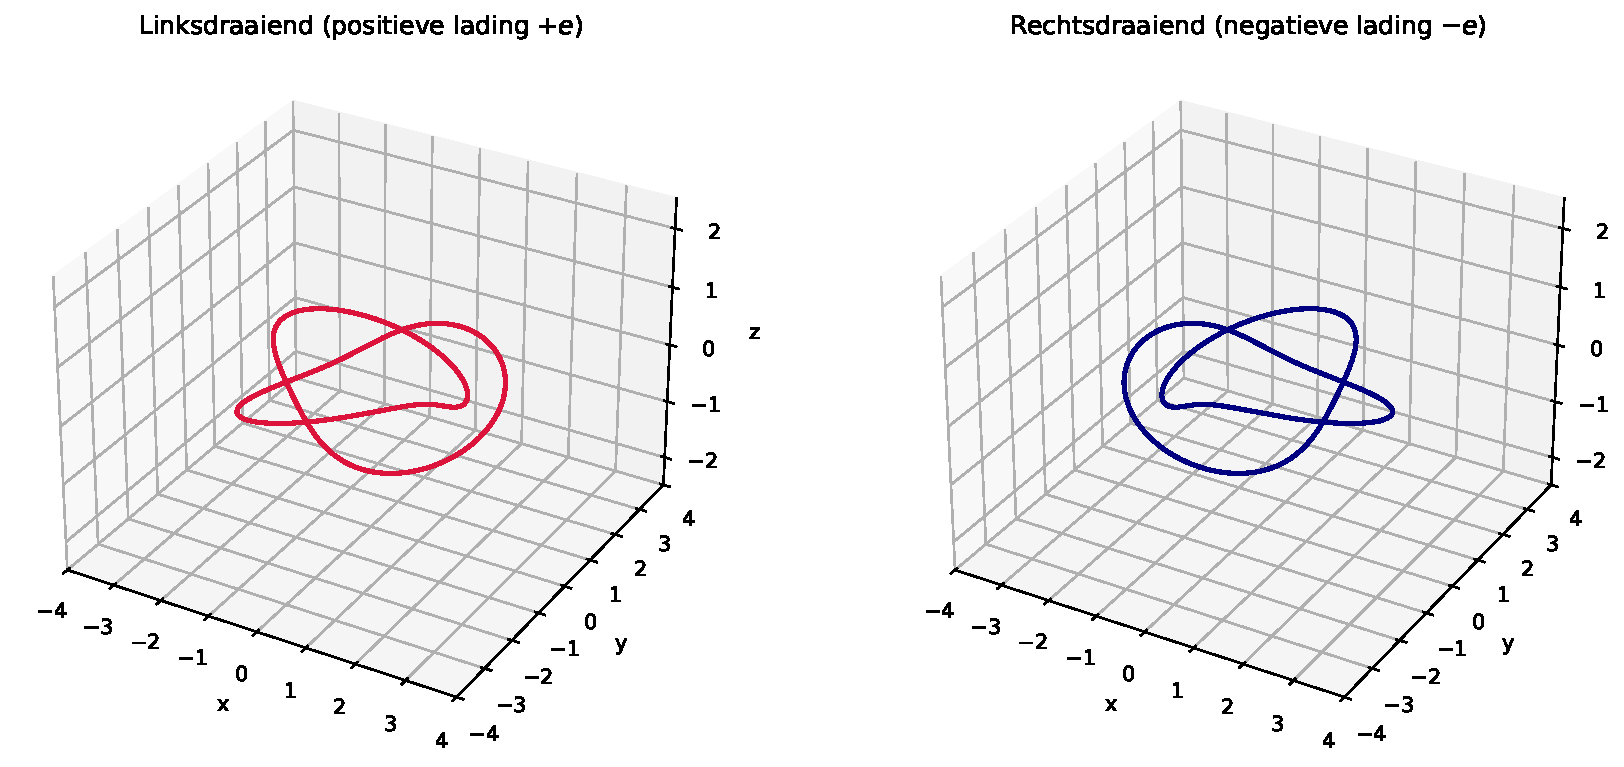
\includegraphics[width=0.8\textwidth]{../6_swirlRichting}
    \caption{Linksdraaiende en rechtsdraaiende vortexknopen. Volgens VAM bepaalt de draairichting de waargenomen elektrische lading.}
    \label{fig:swirl_lading}
\end{figure}

Lading daarentegen wordt geassocieerd met de heliciteit oriëntatie. Een vortexknoop heeft een chirale eigenschap – een onderscheid tussen links- en rechtsdraaiende werveling. VAM identificeert dit met positieve vs. negatieve elektrische lading. Concreet: een knoop met een bepaalde heliciteitsrichting induceert een vectorpotentiaal in de æther die overeenkomt met een elektromagnetisch veld. Hierdoor gedraagt de wervelknoop zich als een geladen deeltje, hoewel er in het model geen fundamentele "ladingsdrager" is behalve de draaiende æther zelf.

VAM verklaart daarmee ook waarom lading gekwantiseerd is: heliciteit in een knoop kan niet continu variëren maar is gebonden aan integer linking (of een vaste verhouding daartussen). Bijvoorbeeld, de trefoil met $L_k=3$ genereert één elementaire ladingeenheid $e$. Dit suggereert dat de elementaire heliciteitseenheid overeenkomt met 1/3e – opvallend gelijk aan de fractiele ladingen van quarks. Inderdaad zou men kunnen zeggen dat de vortexheliciteit verdeeld is in 3 subfluxen (denk aan drie fluxringetjes ineen) die gezamenlijk de knoop vormen, analoog aan de drie quarks in een baryon.

Deze analogie is speculatief maar interessant: een proton-trefoil zou zo gezien kunnen worden als een gebonden toestand van drie vortexquanta (elk met heliciteit 1 en lading $+1/3e$) die topologisch niet afzonderlijk bestaan maar samen één knoop vormen. Dit komt overeen met het standaardmodel waarin drie quarks $(+2/3,+2/3,-1/3)$ de lading +1 van de proton geven – in VAM zijn dit drie onverbrekelijke wervelinkepingen die samen $L_k=3$ maken en zo één ladingeenheid opleveren.

Samengevat ontstaat massa uit de totale energie van het wervelveld, die door $L_k$ wordt gekwantiseerd, en lading uit de heliciteitsrichting van dat veld. De spin van het deeltje tenslotte is gerelateerd aan de interne rotatie van de knoop. Een vortexknoop roteert om zijn eigen kern (met hoeksnelheid $\Omega_k$), wat een angulair momentum geeft. In feite kan men aantonen dat een knoop met heliciteit $H$ een eigen draaimoment draagt proportioneel aan $H$ (via een analoog van de Jefimenko\rqs s oplossingen in de æther). Dit is in lijn met het idee dat spin half (fermionen) corresponderen met vortexknopen die één quantum heliciteit uit de æther \grqq zuigen\textquotedblright (bijv. trefoil $L_k=3$ zou effectief spin 1/2 kunnen geven in de juiste normalisatie), terwijl bosonen wellicht samenhangen met samenstellingen met integer netto heliciteit. Deze interpretatie vereist verdere uitwerking, maar VAM biedt in principe een mechanisme waarbij spin geen fundamenteel puntdeeltje-eigenschap is, maar voortkomt uit de draaiende topologie van de ætherknoop.